\subsection{Confronto tra DCT2 implementata e DCT2 di Scipy}\label{confronto}
Innanzitutto è stato effettuata una verifica sui valori ottenuti dalla dct di nostra implementazione rispetto al vettore fornito nella traccia del progetto.\\
Dopodiché, prima di confrontare le performance della dct2 di \emph{libraryMCS} rispetto a quella fornita da \emph{SciPy.fft}, è stato eseguito un controllo sulla consistenza dei valori ottenuti dalle due librerie a partire da matrici di test, in modo da poter confermare che la dct computata con \emph{SciPy.fft} operasse allo stesso modo rispetto a quanto visto a lezione.\\\\
Il confronto sulle performance prende in considerazione il tempo impiegato da \emph{libraryMCS.dct2V1}, \emph{libraryMCS.dct2V2} e dalla doppia applicazione di \emph{SciPy.fft.dct} per calcolare la trasformazione su 20 matrici quadrate generate casualmente, le cui dimensioni variano da 10x10 a 200x200 con un incremento di 10x10. 
\\\\
In figura \ref{fig:tempiDCT} è possibile osservare il comportamento dalle tre funzioni al crescere delle dimensioni dell'input. Le ascisse rappresentano le dimensioni delle matrici, mentre le ordinate, in scala logaritmica, corrispondono al tempo impiegato.
Le curve nel grafico confermano le previsioni riguardo la complessità computazionale delle diverse implementazioni.\\
Il metodo \emph{dct2V2}, la cui complessità è pari a \emph{O($N^{4}$)}, risulta il meno performante. 
Questo metodo è stato volutamente limitato alle prime 10 matrici a causa dei notevoli tempi richiesti.\\
Il metodo \emph{dct2V1}, di complessità \emph{O($N^{3}$)}, mostra un comportamento nettamente migliore del precedente.\\
Infine \emph{SciPy.fft.dct}, la cui complessità è ridotta a \emph{O($N^{2}$log(N))} per merito della Fast Fourier Transform, ottiene il risultato migliore in assoluto. \\
I tempi effettivi non in scala logaritmica sono consultabili nella tabella \ref{tab:tempiDCT}.

\begin{figure}[H]
    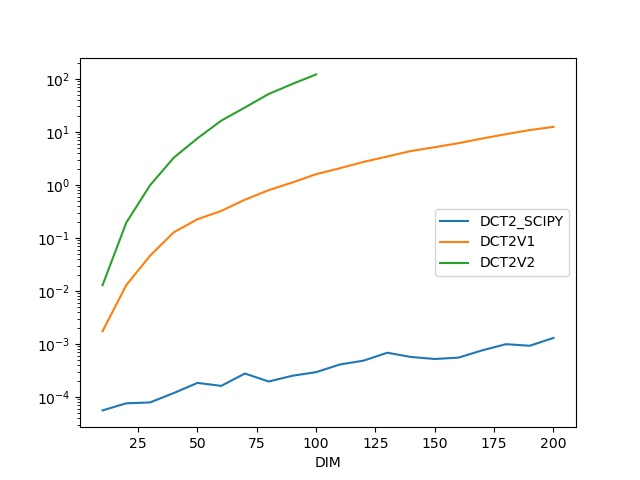
\includegraphics[width=\columnwidth]{tempiDCT}\centering
    \caption{Tempo impiegato dalle diverse implementazioni di dct2 (sulle y in scala logaritmica) all'aumentare delle dimensioni dell'input (sulle x)}\label{fig:tempiDCT}
\end{figure}

\begin{table}[]
    \begin{tabular}{|l|l|l|l|}
    \hline
    \textbf{SciPy} & \textbf{dct2V1} & \textbf{dct2V2} & \textbf{Dim.} \\ \hline
    5.569999999999187e-05 & 0.0017336000000000018 & 0.012775300000000045 & 10 \\
    7.580000000007026e-05 & 0.012813999999999992 & 0.19321499999999991 & 20 \\
    7.869999999998711e-05 & 0.04581029999999997 & 0.9775666000000001 & 30 \\
    0.00011830000000001561 & 0.12703189999999998 & 3.2447316 & 40 \\
    0.0001838000000002893 & 0.22438480000000016 & 7.5267007 & 50 \\
    0.0001614999999990374 & 0.3212653000000003 & 16.198178 & 60 \\
    0.0002761000000006675 & 0.5238236000000001 & 28.738181400000002 & 70 \\
    0.00019520000000028404 & 0.7929004000000006 & 51.56870620000001 & 80 \\
    0.0002507999999892263 & 1.1066644999999937 & 79.8446131 & 90 \\
    0.000293400000003885 & 1.588044999999994 & 120.83413380000002 & 100 \\
    0.00040869999997994455 & 2.0552627000000143 & - & 110 \\
    0.00048359999999547654 & 2.703120599999977 & - & 120 \\
    0.0006816000000071654 & 3.4227569000000244 & - & 130 \\
    0.000566400000025169 & 4.343924700000002 & - & 140 \\
    0.0005194999999957872 & 5.121972200000016 & - & 150 \\
    0.0005508999999506159 & 6.102163299999972 & - & 160 \\
    0.0007562000000120861 & 7.4770121000000245 & - & 170 \\
    0.0009878000000185239 & 9.013939600000015 & - & 180 \\
    0.0009223000000133652 & 10.770630900000015 & - & 190 \\
    0.0012959999999679894 & 12.3887158 & - & 200 \\ \hline
    \end{tabular}
    \caption{Tempi di computazione delle diverse implementazioni di dct2}
    \label{tab:tempiDCT}
\end{table}